

\begin{tikzpicture}[]


\node[anchor=north west, inner sep=0pt] (cpu) at (-6.99, 0){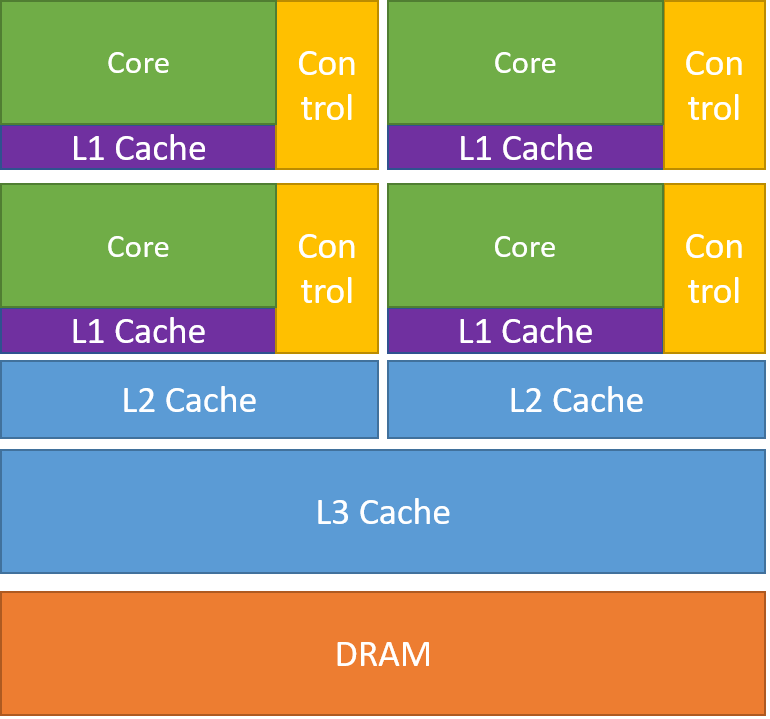
\includegraphics[width=3cm]{figure/session-1/cpu-architecture.png}};
\node[anchor=south] at (cpu.north) {CPU};

\node[anchor=north east, inner sep=0pt] (gpu) at (6.99, 0){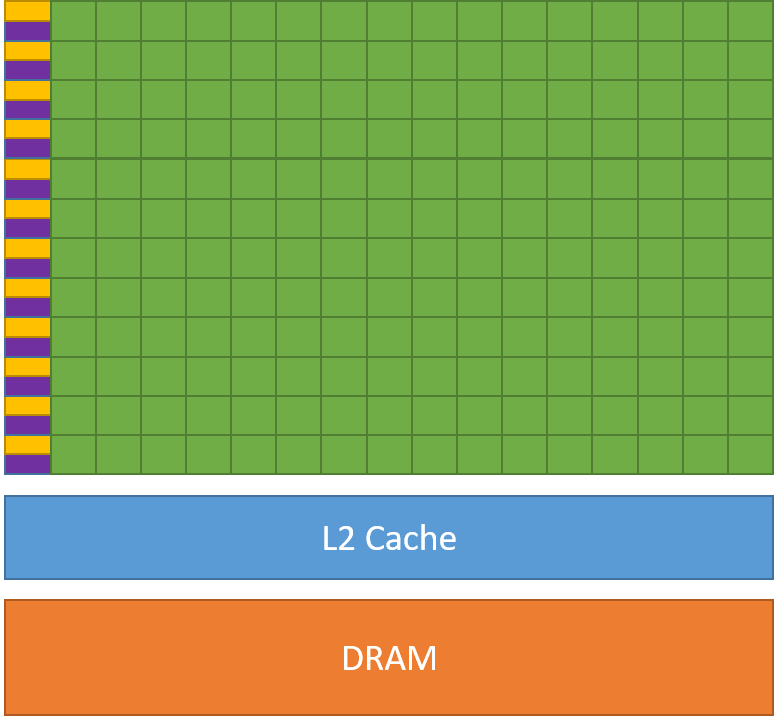
\includegraphics[width=3cm]{figure/session-1/gpu-architecture.png}};
\node[anchor=south] at (gpu.north) {GPU};

\fill[anchor=north, color=black!5!white] (-2.5,0) rectangle ++(5,-2.2);
\fill[anchor=north, color=black!10!white] (-2.5,-2.2) rectangle ++(5,-2.8);
\draw[anchor=north] (-2.5,0) rectangle ++(5,-5);
\node[anchor=south] at (0,0) {code.cpp};


% Top script

\def\topy{-0.35}

\node[anchor=west, align=left, font=\footnotesize] at (-2.4, \topy) {1.};
\node[anchor=west, align=left, font=\footnotesize] at (-2, \topy) {Includes and defines};

\node[anchor=west, align=left, font=\footnotesize] at (-2.4, \topy-0.6) {2.};
\node[anchor=west, align=left, font=\footnotesize] at (-2, \topy-0.6) {CPU functions};
\node[anchor=west, align=left, font=\footnotesize] at (-2, \topy-1.0) {Kernel functions (global)};
\node[anchor=west, align=left, font=\footnotesize, text=OliveGreen] at (-2, \topy-1.4) {GPU functions (device)};



% Bottom script

\def\topy{-2.7}

\node[anchor=west, align=left, font=\footnotesize] at (-2.4, \topy) {3.};
\node[anchor=west, align=left, font=\footnotesize] at (-2, \topy) {Memory alloc. and migration};

\node[anchor=west, align=left, font=\footnotesize] at (-2.4, \topy-0.6) {4.};
\node[anchor=west, align=left, font=\footnotesize] at (-2, \topy-0.6) {Kernel invocation (and timing)};

\node[anchor=west, align=left, font=\footnotesize] at (-2.4, \topy-1.2) {5.};
\node[anchor=west, align=left, font=\footnotesize] at (-2, \topy-1.2) {Memory migration};
\node[anchor=west, align=left, font=\footnotesize] at (-2, \topy-1.6) {(and checking/dumping)};



\draw [decorate, decoration={brace, amplitude=10pt, mirror}] (-2.9,0) -- (-2.9,-5);
% \draw [-{angle 60}] (-3.3, -2.5) -- (-3.8, -2.5);
\node[anchor=center, align=center, font=\footnotesize] at (-5, -3.5) {Compilation/execution \\on the CPU};


\only<2->{
\draw [decorate, decoration={brace, amplitude=10pt}] (1.8,-1.2) -- (1.8,-1.9);
\draw [-{angle 60}] (2.35, -1.55) -- (3.5, -1.55);
\draw [-{angle 60}] (2.1, -2.6) -- (3.5, -2.0);
% \draw [-{angle 60}] (1.6, -4.2) -- (3.5, -2.8);
\draw [-{angle 60}] (1.6, -4.2) -- (3.5, -2.8);
\node[anchor=center, align=center, font=\footnotesize] at (5, -3.5) {Interface to the GPU};
}


\only<3->{
% Bottom script
\draw [-{angle 60}] (-2.4, -3.2) to[out=160, in=-140] (-2.0, -1.45);
\draw [-{angle 60}] (1.45, -1.35) 
to[out=-10, in=90] (1.7, -1.525)
to[out=-90, in=10] (1.3, -1.75);
}


\end{tikzpicture}
